\documentclass[a2paper]{article}

\usepackage{siunitx}
\usepackage{tikz}
\usepackage{amsmath}
\usepackage{geometry}
% \usepackage{showframe}

\geometry{a2paper,margin=0.5in}
\pagestyle{empty}

\begin{document}
\thispagestyle{empty}

\begin{figure}[h!]
\begin{tikzpicture}
\node[anchor=south west,inner sep=0] at (0.2,-5.0) 
{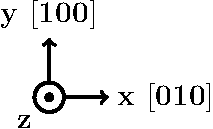
\includegraphics[width=0.30\textwidth]{arrows1}};
\node[anchor=south west,inner sep=0] at (0.2,-0.3) 
{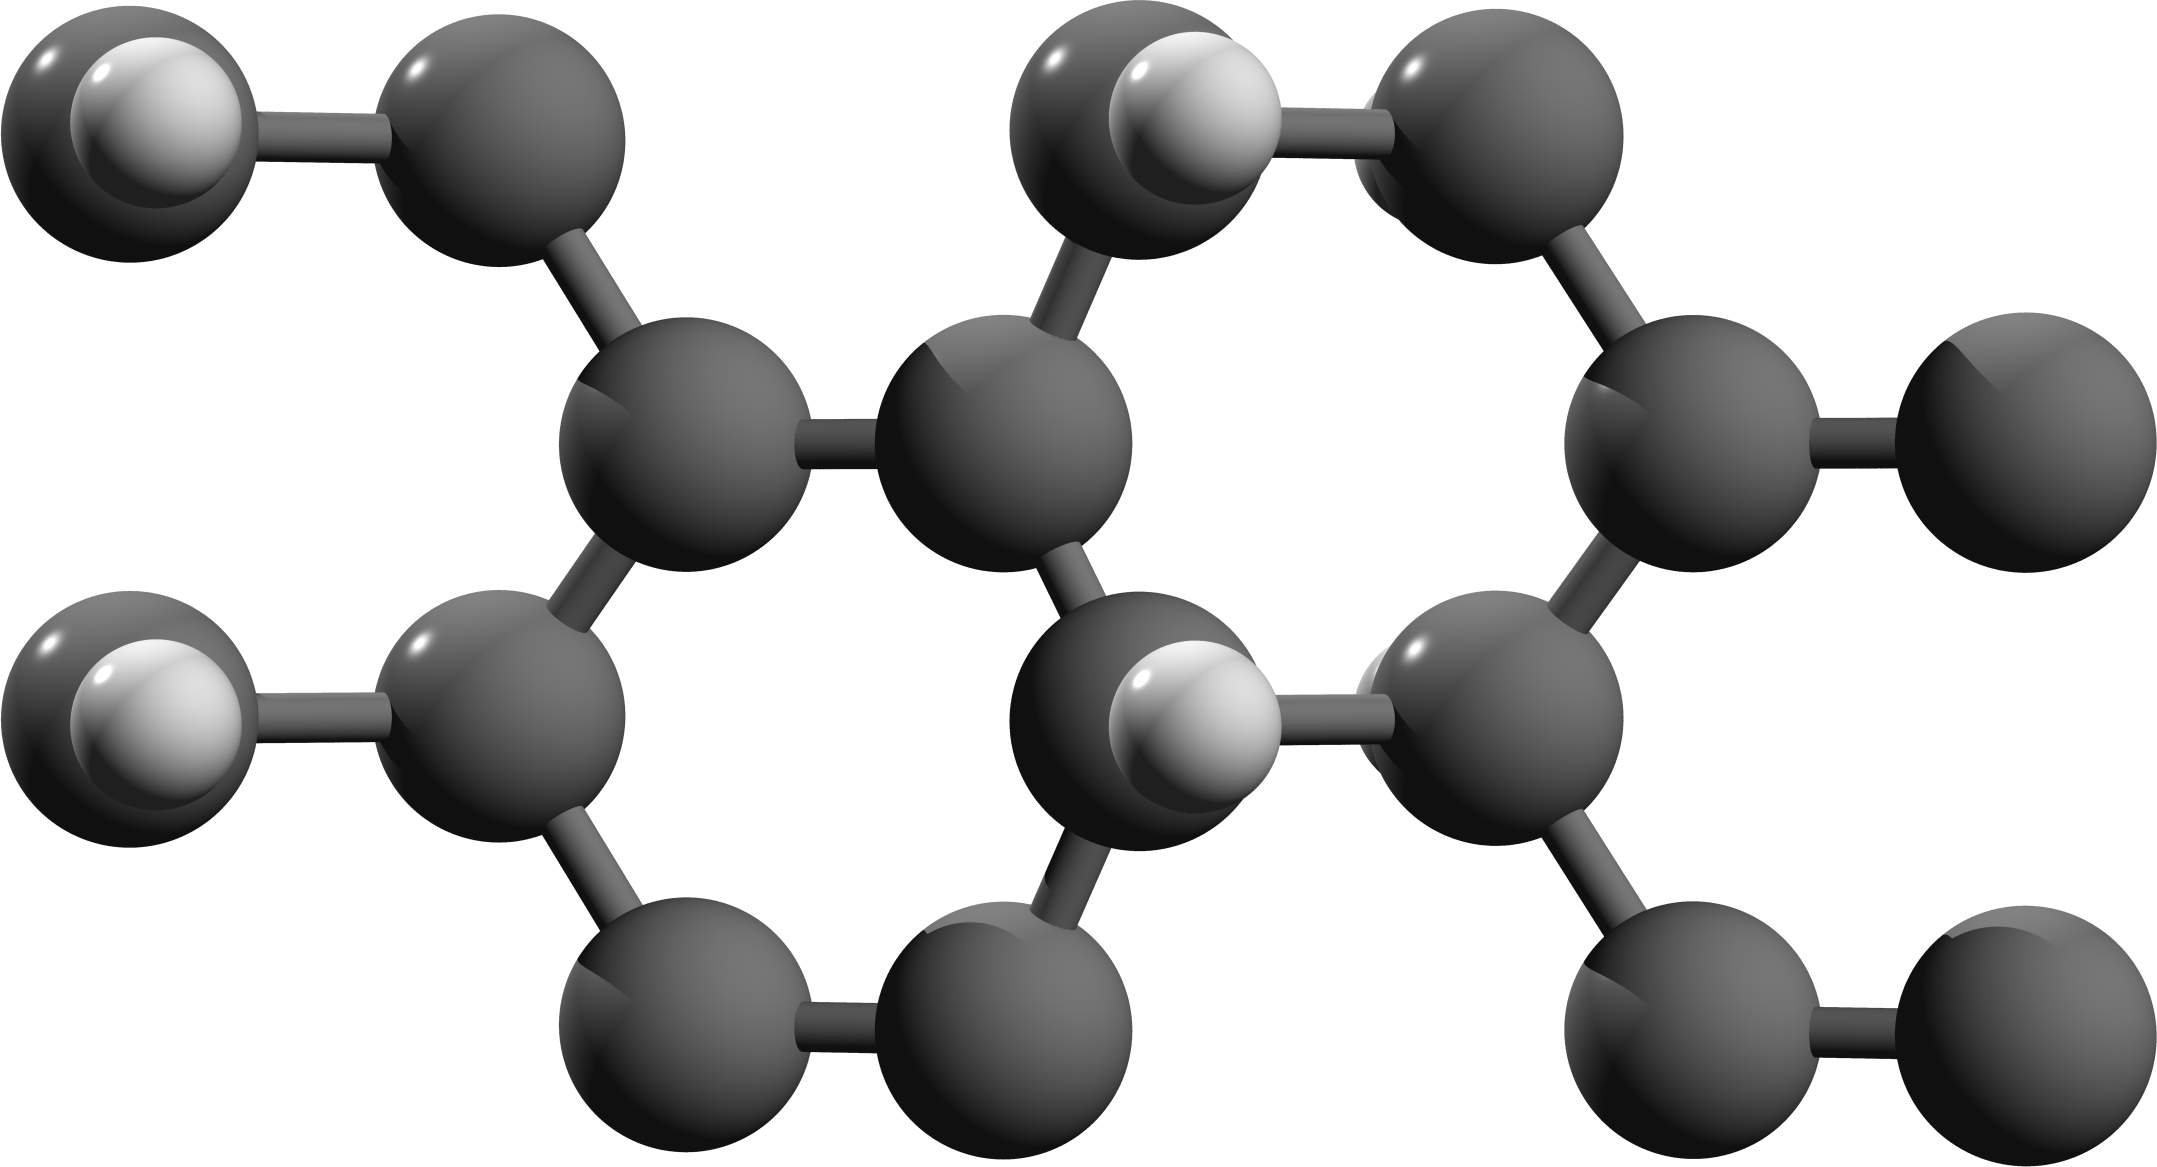
\includegraphics[width=\textwidth]{alt1}};
\draw [line width=2.00mm, red, -> ] (2.80,07.50) -- (2.80,19.00) 
node [right] {};
\draw [line width=2.00mm, red, -> ] (2.80,07.50) -- (22.00,07.50) 
node [right] {};
\draw [line width=2.00mm, red, dashed ] (22.00,07.50) -- (22.00,19.00) 
node [right] {};
\draw [line width=2.00mm, red, dashed ] (2.80,19.00) -- (22.00,19.00) 
node [right] {};
\node[anchor=south west,inner sep=0] at (0.2,-34.0) 
{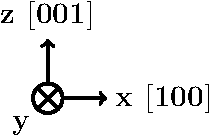
\includegraphics[width=0.30\textwidth]{arrows2}};
\node[anchor=south west,inner sep=0] at (0.2,-24.6) 
{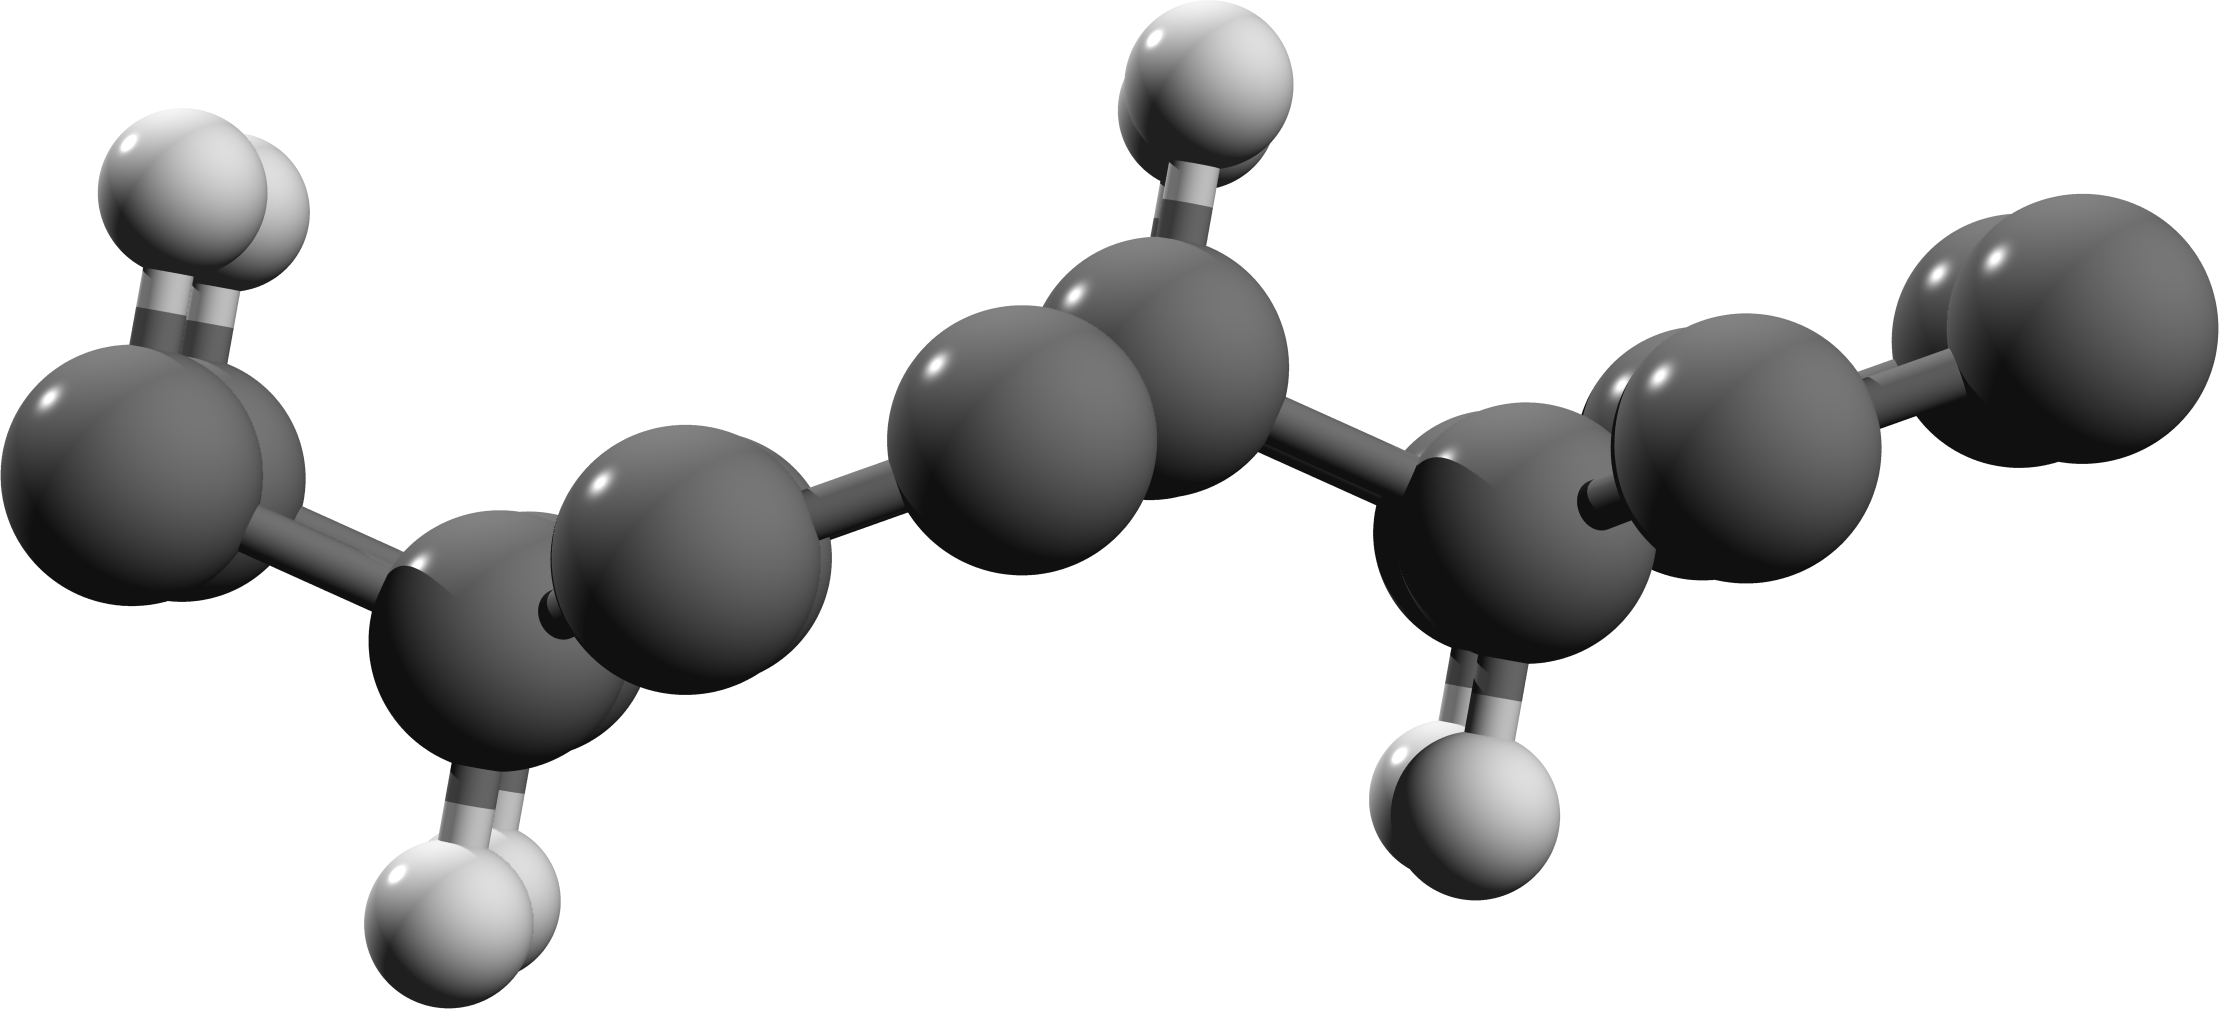
\includegraphics[width=\textwidth]{alt2}};
\end{tikzpicture}
\end{figure}

\end{document}
/Users/reinaldo/Desktop/structures/fig1.tex
